\documentclass{article}
\usepackage{graphicx} % Required for inserting images
\usepackage{ctex}
\usepackage{graphicx}
\usepackage{xcolor}
\usepackage{titlesec}
\usepackage{amsmath}
\usepackage{amssymb}
\usepackage{listings}

\lstset{
  language=C,
  basicstyle=\ttfamily\footnotesize,
  keywordstyle=\color{blue},
  commentstyle=\color{gray},
  stringstyle=\color{red},
  numbers=left,
  numberstyle=\tiny,
  stepnumber=1,
  numbersep=5pt,
  showstringspaces=false,
  breaklines=true,
  frame=single,
  captionpos=b
}

\titleformat{\section}{\Large\bfseries\color{black}}{\thesection}{1em}{}
\titleformat{\subsection}{\large\bfseries\color{black}}{\thesubsection}{1em}{}

\title{信号分离装置}
\author{徐圣毅，何衍宁，向阳，陈信均}
\date{2025年 6月6日}


\begin{document}

\maketitle
\quad
关键词： 信号分离；实时信号同步；离散傅里叶变换；DAC 输出 

\section{项目介绍}

\subsection{任务}
设计并制作信号分离装置，如图所示。一台双路输出信号源输出 2 路周期信号 A 和 B（频率范围：20kHz~100kHz，且 $f_A < f_B$；峰峰值均为 1V），经增益为 1 的加法器产生混合信号 C，信号 C 通过分离电路分离出信号 A' 和 B'。信号 A' 和 B' 相比信号 A 和 B 波形无失真，A' 和 A、B' 和 B 的波形在示波器上能连续稳定同频显示。



\subsection{基本要求}

\begin{enumerate}
    \item 制作增益为 1 的加法器，实现 $C = A + B$。
    \item 信号 $A$ 和 $B$ 均为正弦波，$f_A = 50\,\mathrm{kHz}$，$f_B = 100\,\mathrm{kHz}$。装置能正确分离出信号 $A'$ 和 $B'$，且峰峰值均不小于 1V。
    \item 信号 $A$ 和 $B$ 均为正弦波，频率分别为 10kHz 的整数倍。装置能正确分离出信号 $A'$ 和 $B'$，且峰峰值均不小于 1V。
\end{enumerate}


\subsection{发挥部分}
\begin{enumerate}
    \item 信号 $A$ 和 $B$ 分别为正弦波或三角波，频率分别为 5kHz 的整数倍。装置能正确分离出信号 $A'$ 和 $B'$，且峰峰值均不小于 1V。
    \item 信号 $A$ 和 $B$ 分别为正弦波或方波，频率分别为 5kHz 的整数倍。装置能正确分离出信号 $A'$ 和 $B'$，且峰峰值均不小于 1V。
    \item 通过外接串口，使用解析数据成线的软件得到频谱，来分析其正确性，方便进行中间串口的调试。
\end{enumerate}

\section{系统方案}

\begin{figure}[h]
    \centering
    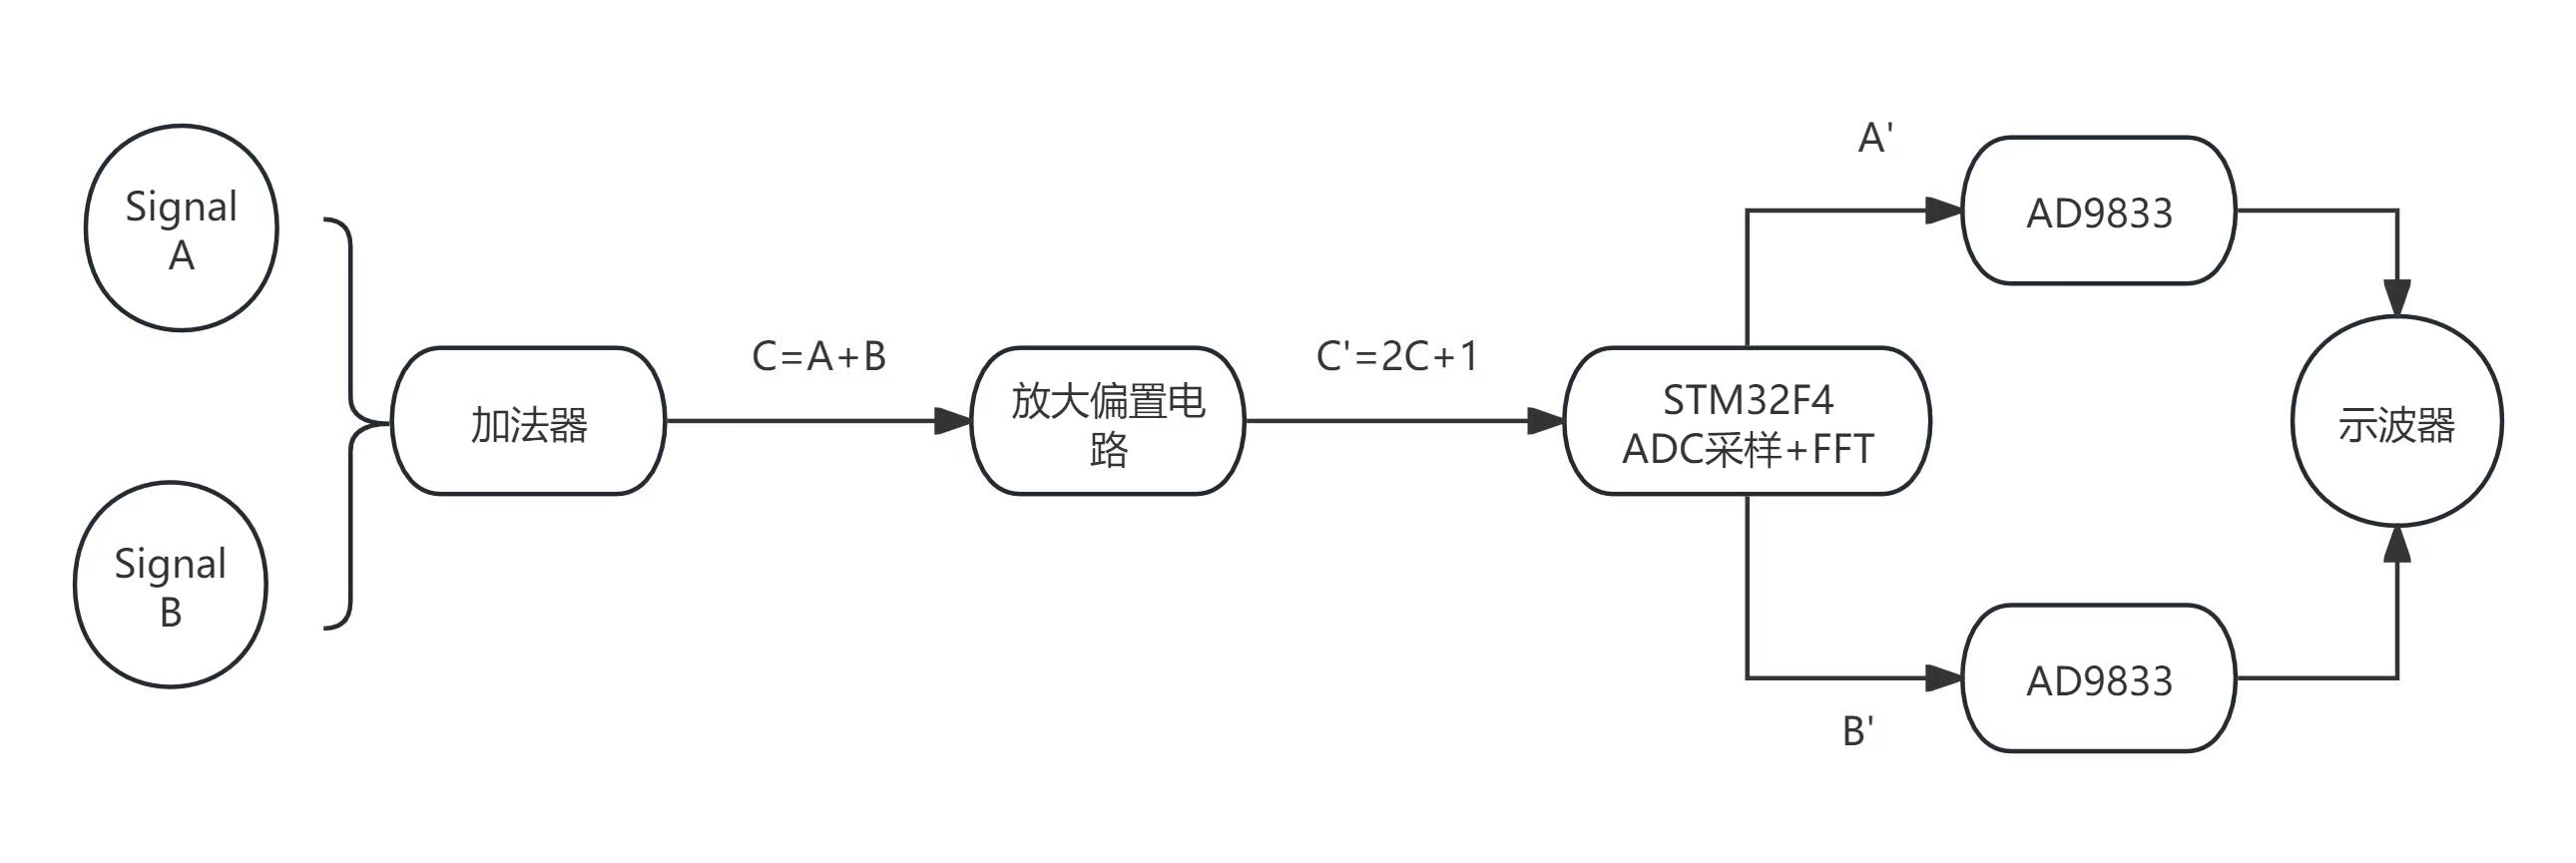
\includegraphics[width=1.0\textwidth]{figure/figure1.jpg} % 替换为您的图片文件名
    \caption{设计思路图}
    \label{fig:example}
\end{figure}

\subsection{设计思路}
信号发生器输出两路信号，经过加法器混合后，利用单片机内置外设ADC对混合信号进行采样，采样时为防止非周期采样窗口，加入采样窗口函数汉明窗，在单片机内部利用FPU进行高精度FFT运算，实现时域到频域转换，分离出两个频率。根据理论指导，利用频域峰值分析频率对应信号波形。将分析得到的信号波形，频率传入DDS，使其输出两路信号，实现分离。
\subsection{主要设计模块}
\begin{enumerate}
\subsubsection{信号源与输入部分}
\begin{enumerate}
\item 信号发生器：产生条件中的A,B信号源，作为调制使用。
\item 模拟加法器模块：
\\1.该模块是两路加法器，将信号发生器产生的信号A和B进行线性叠加，输出一个混合信号$C = A + B$。
\\2.该加法器有运算放大器配置如LM324、TL084等。
\\3.接口：
\\IN1,IN2:接入来自信号发生器的输入信号A,B。
\\OUT:加法结果输出端。
\\V+,V-:接运放的正电源和负电源，分别接+V和-V电压。
\\GND:接地端口。
\\4.说明：加法器为全模拟信号路径，无延迟、无采样误差。运放要对称供电，即使用±电源模块，否则输出可能失真或裁剪。
\end{enumerate}    

\subsubsection{信号处理与分离部分}
\begin{enumerate}
\item 该部分可以选择STM32F1核心板和F4核心板，但由于F1性能没那么好，主时钟频率为72MHZ，F4性能较好，有专门用于浮点数计算的FPU，且主时钟为168MHZ，因此这里我们选择F4核心板。
\item STM32F407ZGT6核心板模块：
\\1.ADC采样模块：
\\STM32F407 内部集成 3 个 12 位 ADC（ADC1、ADC2、ADC3），每个可独立采样。将模拟信号$C' = 2C + 1$转换为数字信号,在使用ADC1 采集经加法放大偏置后的信号 C′，进行频谱分析。通过设置其采样周期、分辨率、触发方式（定时器或DMA），实现稳定、快速采样。
\\2.信号加窗模块:
\\2.1对原始 ADC 采样数据加窗，避免 FFT 运算中由于非周期截断造成的频谱泄露现象。其中加窗函数有如汉明窗（Hamming）、汉宁窗（Hanning）等。这里我们使用汉宁窗。
\\2.2汉明窗的作用：在实际采样中，我们通常只能采集一个有限时间长度的信号段（即所谓截断信号）。这种截断会引发频谱泄漏，此时FFT 会误判频率分量，出现频谱能量扩散，导致分析精度降低。为减轻泄漏影响，需要对信号乘以“窗函数”，让信号在两端平滑过渡（趋近于零），从而减少跳变引起的高频泄漏。因此在窗函数中，汉明窗属于“平滑窗”，对主瓣宽度与旁瓣抑制有较好平衡。相比矩形窗（直接截断），它能有效降低旁瓣（频谱泄漏）但稍微扩大主瓣（频率分辨率略降低）。是典型的用于一般频谱分析的窗函数。
\\2.3理论公式依据：
\begin{equation}
w(n) = 0.54 - 0.46 \cos\left(\frac{2\pi n}{N-1}\right), \quad 0 \leq n \leq N-1
\end{equation}
\\$w(n)$：是第n个窗函数的系数。
\\N：窗口的总长度（通常为你的 FFT 点数，例如 256、512、1024）。
\\n：当前采样点索引。

\\3.频谱分析模块：
\\通过快速傅里叶变换（FFT）运算,将时间域的混合信号$C'(t)$转换为频域信号$F(f)$，识别其中包含的两个频率成分。使用 STM32的FPU（浮点运算单元）+CMSIS DSP库，调用$arm-cfft-f32()$完成FFT。且必须使用\( 2^N \)点 FFT, 如 256, 512, 1024。其中FFT分辨率为\(\Delta f = \frac{f_s}{N}\)，其中 \( f_s \) 为采样频率，\( N \) 为采样点数。
\\4.峰值检测模块：
\\对 FFT 得到的幅度谱进行最大值检测，找出两个主频率分量，这两个频率即为信号 A 与 B 原始频率。计算实际频率：\begin{equation}
f = \frac{\text{index} \cdot f_s}{N}
\end{equation}其中最小分辨率受采样频率和点数影响，此步骤对后续 DDS 控制非常关键。同时我们也需要解决某一信号频谱存在多个比其他信号峰值还要大的情况，这也是我们实际中遇到的问题。
\\5.DDS控制模块：
\\根据分析出的两个频率，控制两个AD9833，输出对应波形，即信号$A’$与$B’$。STM32 使用 SPI 接口向 AD9833 写入频率控制字：\begin{equation}
\text{FreqWord} = \frac{f_{\text{out}} \cdot 2^{28}}{\text{MCLK}}
\end{equation}通过写 SPI 数据方式控制输出频率，实现对原始信号A、B的频率还原。

\\6.串口调试模块：
\\通过串口将采样数据、FFT结果、频率值发送到电脑上位机显示或调试。使用 USART1（PA9/PA10），串口助手查看 FFT 频率、原始波形、调试信息。这也是哦我们的发挥部分之一，使用串口将频谱在电脑上显示出来，方便后续调试。
\\7.时钟与触发模块：
\\STM32主频（168MHz）经过配置可稳定控制 ADC 的采样频率。同时使用定时器+DMA 触发ADC可以保证等间隔采样。
\end{enumerate} 



\subsubsection{电源部分}
\begin{enumerate}
电源部分我们选择多路线性AC-DC正负电源，其可有效降低:地环路噪声,数字高频开关干扰，模拟信号漂移。同时多通道供电器可以实现：单独控制每一路的电压和电流限幅，对比不同模块在不同电压下的响应行为（如AD9833 3.3V vs 5V），快速排查问题（如某模块不上电是否是电源故障）。有效防止了模拟/数字地耦合，电流拉升不足,串扰，启动顺序等问题。
\end{enumerate}    


\end{enumerate}

\subsection{主要算法思路}
\begin{enumerate}

\item STM32F407ZGT6：主频 168\,MHz，APB1 时钟为 42\,MHz，APB2 时钟为 84\,MHz。
\\由于 ADC1 挂载在 APB2 总线上，因此其时钟源为 APB2CLK，即 84\,MHz。

\item ADC1 配置：ADC 时钟分频器（Prescaler）可选 2、4、6、8，为满足 ADCCLK $\leq$ 36\,MHz，选择 Prescaler 为 4：

\begin{equation}
f_{\text{ADCCLK}} = \frac{f_{\text{APB2CLK}}}{\text{Prescaler}} = \frac{84\,\text{MHz}}{4} = 21\,\text{MHz}
\end{equation}

\item 因此，ADC 时钟频率为：

\begin{equation}
f_{\text{ADC}} = \frac{1}{T_{\text{ADC}}} = 21\,\text{MHz}
\end{equation}


\item 由采样配置公式：
\begin{equation}
T_{\text{sample}} = T_{\text{conv}} + T_{\text{read}} \quad (\text{采样周期} = \text{转换时间} + \text{读取时间})
\end{equation}

\item 由于我们开启DMA转运，我们可以进行下面推导：

\begin{equation}
T_{\text{read}} \approx 0
\end{equation}

\begin{equation}
T_{\text{sample}} = T_{\text{conv}} 
\end{equation}

\begin{equation}
T_{\text{conv}} = T_{\text{maintain}} + T_{\text{resolution}} \quad (\text{转换时间} = \text{采样保持} + \text{分辨率转换})
\end{equation}

\begin{equation}
T_{\text{sample}} = T_{\text{maintain}} + T_{\text{resolution}} 
\end{equation}

\begin{equation}
T_{\text{maintain}} = n_1 \cdot T_{\text{ADC}}
\end{equation}

\begin{equation}
T_{\text{resolution}} = n_2 \cdot T_{\text{ADC}} \quad (\text{各自时长} = \text{周期数} \cdot \text{ADC单周期时长})
\end{equation}

\begin{equation}
T_{\text{sample}} = (n_1 + n_2) \cdot T_{\text{ADC}}
\end{equation}

\begin{equation}
f_{\text{sample}} = \frac{f_{\text{ADC}}}{(n_1 + n_2)}
\end{equation}

\item 上述可配参数：
\\ADC-Prescalar=4,6,8（84/2=42>36）
\\n1=3,15,28,56,84...（后面用不到）
\\n2=15,13,11,9

\item FFT 算法：
\\对长度为 $K$ 的一维数组进行快速傅里叶变换（FFT），得到同样大小的频域数组。数组中第 $k$ 个元素代表第 $k \cdot R_{\text{frequency}}$ 赫兹处的频率分量幅值，其中 $a[0]$ 对应直流分量（0\,Hz）。

\begin{equation}
R_{\text{frequency}} = \frac{f_{\text{sample}}}{K}
\end{equation}

\\即频率分辨率由采样频率和点数 $K$ 决定。由于计算机运算特性，建议选取 $K = 2^N$。

\item 有关 $n_1$、$n_2$、$N$ 的推导：

\begin{equation}
\text{频率范围约束条件:} \quad (K - 1) \cdot R_{\text{frequency}} \geq f_{\text{max}}
\end{equation}

\begin{equation}
\text{奈奎斯特采样定理:} \quad f_{\text{sample}} \geq 2 f_{\text{max}}
\end{equation}

\begin{equation}
\text{频率分辨率要求:} \quad R_{\text{frequency}} = 10^m
\end{equation}

\begin{equation}
f_{\text{sample}} = \frac{21 \times 10^6}{n_1 + n_2}
\end{equation}

\begin{equation}
\frac{21 \times 10^6}{n_1 + n_2} \geq 2 \times 100 \times 10^3
\end{equation}

\begin{equation}
R_{\text{frequency}} = \frac{f_{\text{sample}}}{2^N} = \frac{21 \times 10^6}{2^N (n_1 + n_2)} = 10^m
\end{equation}

\item 最终选定参数如下：

\begin{itemize}
  \item ADC 时钟预分频器（Prescaler）：4
  \item 定时器周期计数参数：$n_1 = 28$, $n_2 = 13$
  \item FFT 点数指数：$N = 9$
  \item FFT 点数：$K = 2^N = 512$
\end{itemize}

\item 验证其合理性：

\begin{equation}
f_{\text{sample}} = \frac{2 \times 10^6}{41} \approx 500 \, \text{kHz} > 200 \, \text{kHz}
\end{equation}

\begin{equation}
R_{frequency} = \frac{f_{sample}}{k} = \frac{21 \times 10^6}{41 \times 512} \approx 1000.381 \approx 1kHz
\end{equation}

\begin{equation}
a[0] \leftrightharpoons 0 \, \text{Hz}, \quad
a[1] \leftrightharpoons 1 \, \text{kHz}, \quad
a[2] \leftrightharpoons 2 \, \text{kHz}, \quad
\ldots, \quad
a[100] \leftrightharpoons 100 \, \text{kHz}
\end{equation}

\item 在计算得到所有数据后，我们仅需对数组 \( a[512] \) 中的 \( a[1] \) 至 \( a[100] \) 进行查找（其中 \( a[0] \) 表示直流分量），找出值最大的两个下标 \( \text{index}_{\text{max1}} \) 和 \( \text{index}_{\text{max2}} \)，则：

\begin{equation}
f_A = (\text{index}_{\text{max2}}) \cdot K_{h3}, \quad f_B = (\text{index}_{\text{max1}}) \cdot K_{h2}
\end{equation}

\end{enumerate}


\end{enumerate}

\subsection{STM32主程序文件}

\begin{enumerate}
    \item STM32主程序 \texttt{main.c} 代码如下所示，主要完成了ADC采样、汉明窗加权、FFT分析、频谱峰值提取与频率还原（使用AD9833模块）等操作。
\end{enumerate}

\begin{lstlisting}[language=C, caption=main.c 主程序文件]
#include "stm32f4xx.h"                  // STM32F4 外设头文件
#include "adc.h"                        // 自定义ADC初始化模块
#include "usart.h"                      // 串口通信模块
#include <math.h>                       // 数学函数
#include "arm_math.h"                   // CMSIS DSP库
#include "arm_const_structs.h"          // CMSIS 结构体
#include "delay.h"                      // 延时函数
#include "tim.h"                        // 定时器初始化
#include "AD9833.h"                     // AD9833 波形合成器控制库
#include <stdlib.h>
#include <stdio.h>

extern uint16_t ADC_ConvertedValue[512]; // ADC采集结果数组（外部定义）

#define FFT_SIZE 512                     // FFT窗口大小
float32_t hamming_window[FFT_SIZE] = {0};  // 汉明窗数组
float32_t window_gain = 1.0f;             // 窗函数增益因子
float32_t fft_input[2 * FFT_SIZE] = {0};  // FFT输入（复数）
float32_t fft_output[FFT_SIZE / 2] = {0}; // FFT输出（幅度谱）
float32_t adc_buffer[FFT_SIZE] = {0};     // 电压转换后的ADC缓存

int index1 = 0, index2 = 0;
float32_t max1 = -1.0f, max2 = -1.0f;
int wave_type_and_req = 0;

// 定时器中断服务函数，用于测试
void TIM1_UP_TIM10_IRQHandler(void)
{
    if (TIM_GetITStatus(TIM1, TIM_IT_Update) != RESET)
    {
        printf("%d\r\n", 100); // 输出测试信息
        TIM_ClearITPendingBit(TIM1, TIM_IT_Update);
    }
}

// 初始化汉明窗
void init_hamming_window(void) 
{
    float32_t sum = 0.0f;
    for (int i = 0; i < FFT_SIZE; i++) {
        hamming_window[i] = 0.54f - 0.46f * arm_cos_f32(2.0f * PI * i / (FFT_SIZE - 1));
        sum += hamming_window[i];
    }
    window_gain = sum / FFT_SIZE; // 计算窗函数增益
}

// 准备FFT输入数据
void prepare_fft_input(void) 
{
    for (int i = 0; i < FFT_SIZE; i++) {
        adc_buffer[i] = (float32_t)ADC_ConvertedValue[i] * 3.3f / 4096.0f; // 数字量转电压
        float32_t windowed = adc_buffer[i] * hamming_window[i]; // 加窗
        fft_input[2 * i] = windowed;    // 实部
        fft_input[2 * i + 1] = 0.0f;    // 虚部置0
    }
}

// 执行FFT分析
void do_fft_analysis(void) 
{
    arm_cfft_f32(&arm_cfft_sR_f32_len512, fft_input, 0, 1); // FFT变换
    float32_t fft_full[FFT_SIZE];
    arm_cmplx_mag_f32(fft_input, fft_full, FFT_SIZE); // 复数幅度计算

    fft_output[0] = fft_full[0] / (FFT_SIZE * window_gain); // 直流分量
    for (int i = 1; i < FFT_SIZE / 2; i++) {
        fft_output[i] = fft_full[i] * 2.0f / (FFT_SIZE * window_gain); // 归一化有效频率成分
    }
}

// 找出频谱中幅值最大的两个频点
void find_top2_peaks_in_range(int start, int end) 
{
    max1 = -1.0f; max2 = -1.0f; index1 = 0; index2 = 0;

    for (int i = start; i <= end; i++) {
        if (fft_output[i] > max1) {
            max1 = fft_output[i];
            index1 = i;
        }
    }
    for (int i = start; i <= end; i++) {
        if (abs(i - index1) >= 5 && fft_output[i] > max2) {
            max2 = fft_output[i];
            index2 = i;
        }
    }
}

// 发送频率与波形信息至 AD9833
void send_type_and_frequency(void)
{
    float32_t difference = max1 - max2;
    float32_t ratio = max1 / max2;

    if (ratio >= 1.2f) {
        if (index1 > index2) {
            AD9833_WaveSeting_B((double)index1 * 1000, 0, SIN_WAVE, 0);
            AD9833_WaveSeting_A((double)index2 * 1000, 0, TRI_WAVE, 0);
            wave_type_and_req = 1;
        } else {
            AD9833_WaveSeting_B((double)index2 * 1000, 0, TRI_WAVE, 0);
            AD9833_WaveSeting_A((double)index1 * 1000, 0, SIN_WAVE, 0);
            wave_type_and_req = 2;
        }
    } else {
        if (max1 >= 0.4f) {
            if (index1 > index2) {
                AD9833_WaveSeting_B((double)index1 * 1000, 0, SIN_WAVE, 0);
                AD9833_WaveSeting_A((double)index2 * 1000, 0, SIN_WAVE, 0);
                wave_type_and_req = 3;
            } else {
                AD9833_WaveSeting_B((double)index2 * 1000, 0, SIN_WAVE, 0);
                AD9833_WaveSeting_A((double)index1 * 1000, 0, SIN_WAVE, 0);
                wave_type_and_req = 4;
            }
        } else {
            if (index1 > index2) {
                AD9833_WaveSeting_B((double)index1 * 1000, 0, TRI_WAVE, 0);
                AD9833_WaveSeting_A((double)index2 * 1000, 0, TRI_WAVE, 0);
                wave_type_and_req = 5;
            } else {
                AD9833_WaveSeting_B((double)index2 * 1000, 0, TRI_WAVE, 0);
                AD9833_WaveSeting_A((double)index1 * 1000, 0, TRI_WAVE, 0);
                wave_type_and_req = 6;
            }
        }
    }
}

int main(void)
{
    Debug_USART_Config();       // 初始化串口
    ADC1_Init();                // 初始化ADC
    Delay_ms(500);              // 上电延迟
    init_hamming_window();      // 初始化窗函数
    prepare_fft_input();        // 准备FFT输入
    do_fft_analysis();          // 执行FFT
    find_top2_peaks_in_range(10, 110); // 查找峰值
    AD9833_Init_GPIO();         // 初始化AD9833通信接口
    send_type_and_frequency();  // 根据FFT结果设定波形参数

    while(1)
    {
        for (int i = 0; i < FFT_SIZE/2; i++) {
            printf("%f\r\n", fft_output[i]); // 打印频谱数据
        }
    }
}
\end{lstlisting}

\section{实验结果与总结}
在最后的实验测试中，我们成功完成了三个基本要求，增益为1的加法器，不同频率下正弦波与正弦波的信号分离，同时满足峰峰值。我们也成功分离了正弦波和三角波，满足频率和峰值范围，而且通过串口数据的获取，成功打印出频谱，让我们的整个信号处理过程变得非常直观清晰，且极大的方便了我们的调试过程。在调试过程中我们也遇到了许多问题，其中最主要的有两个，第一个是在部署STM32的DSP库，调用fft函数时，发现调用函数后陷入长时间等待。一开始以为是窗口函数导致出错，在通过逐项排查之后,我们发现是STM32F4默认的内存和堆栈配置错误，由于fft算法需要比较大量的临时内存用于存放大量浮点结果，因此通过在start up 文件中替换相关底层参数设置之后，顺利运行FFT函数。第二个是峰值比例判定/差值判定的选择，在利用峰值判断法时，虽然理论上简洁准确，但是由于实际电路要考虑阻抗等问题，实际在利用峰值判断信号是三角波还是正弦波的时候，判据具体数值需要实际标定。因此我们做了大量测试之后，得出一个结果，max1/max2的大于某个值是正弦波、三角波,小于某个值就是两个同类型波，这个值理论上是1.25，实际上是小于这个值的，具体多少要标定一下，在上电之后看频谱调整。

\end{document}
